\subsubsection{Short term}
\label{subsubsec:short-res}

In Table~\ref{tab:short-map-ndcg-table} are reported the \ac{nDCG} and \ac{MAP} values obtained from the submitted runs on the short term collection, while in Figure~\ref{fig:precision-recall-curve-short-term} is reported the interpolated Precision-Recall curve. Comparing these results with the ones obtained on heldout, shown in Table~\ref{tab:heldout-map-ndcg-table} and Figure~\ref{fig:precision-recall-curve-heldout} respectively, we can see that every run has \emph{increased} its performances. This improvement was \emph{not expected} since the performances should tend to drop over time. This can be due to the fact that this set of runs is almost 9 times bigger than the heldout, therefore we can consider the mean measures obtained to be more \emph{reliable} than the ones on the heldout collection.

Observing the \ac{nDCG} and \ac{AP} boxplots, shown in Figure~\ref{fig:short-boxplot}, we can notice that the runs performed on the French collection have a similar structure in terms of median values and interquartile ranges. We can also notice that in the \ac{AP} boxplot the fr\_1 run has a longer whisker, while the others show the presence of outliers.

From the ANOVA2 analysis, which results are reported in Table~\ref{tab:short-anova2}, we can see that $p\textrm{--}value<\alpha$, therefore we \emph{can reject} the null hypothesis. Moreover, from Tukey's \ac{HSD} multiple comparison shown in Figure~\ref{fig:short-hsd}, we can derive that runs fr\_3, fr\_4 can be considered similar, while all the other runs differ from each other.

\begin{table}[tbp]
\caption{\ac{nDCG} and \ac{MAP} values on short term collection}
  \label{tab:short-map-ndcg-table}
    \centering
    \begin{tabular}{|p{0.7\linewidth}|p{0.075\linewidth}|p{0.075\linewidth}|}
	\toprule
	\textbf{Run name} & \textbf{nDCG} & \textbf{MAP} \\
	\midrule
        FADERIC\_French-BM25-Stop50-LightStem-Shingle-Fuzzy-SynCustom-Rerank20W6 & 0.4239 & 0.2665 \\ 
        FADERIC\_French-BM25-Stop50-LightStem-Shingle-Fuzzy-Rerank30 & 0.4145 & 0.2546 \\ 
        FADERIC\_French-BM25-Stop50-LightStem-Shingle-Fuzzy-SynCustom & 0.4034 & 0.2412 \\ 
        FADERIC\_French-BM25Tuned-Stop50-LightStem-Shingle-Fuzzy & 0.4034 & 0.2414 \\ 
        FADERIC\_English-BM25-Stop50-KStem-Shingle-Fuzzy-SynPOS\\-Rerank30 & 0.3296 & 0.1931 \\ 
	\bottomrule
    \end{tabular}
\end{table}

\begin{figure}[tbp]
  \centering
  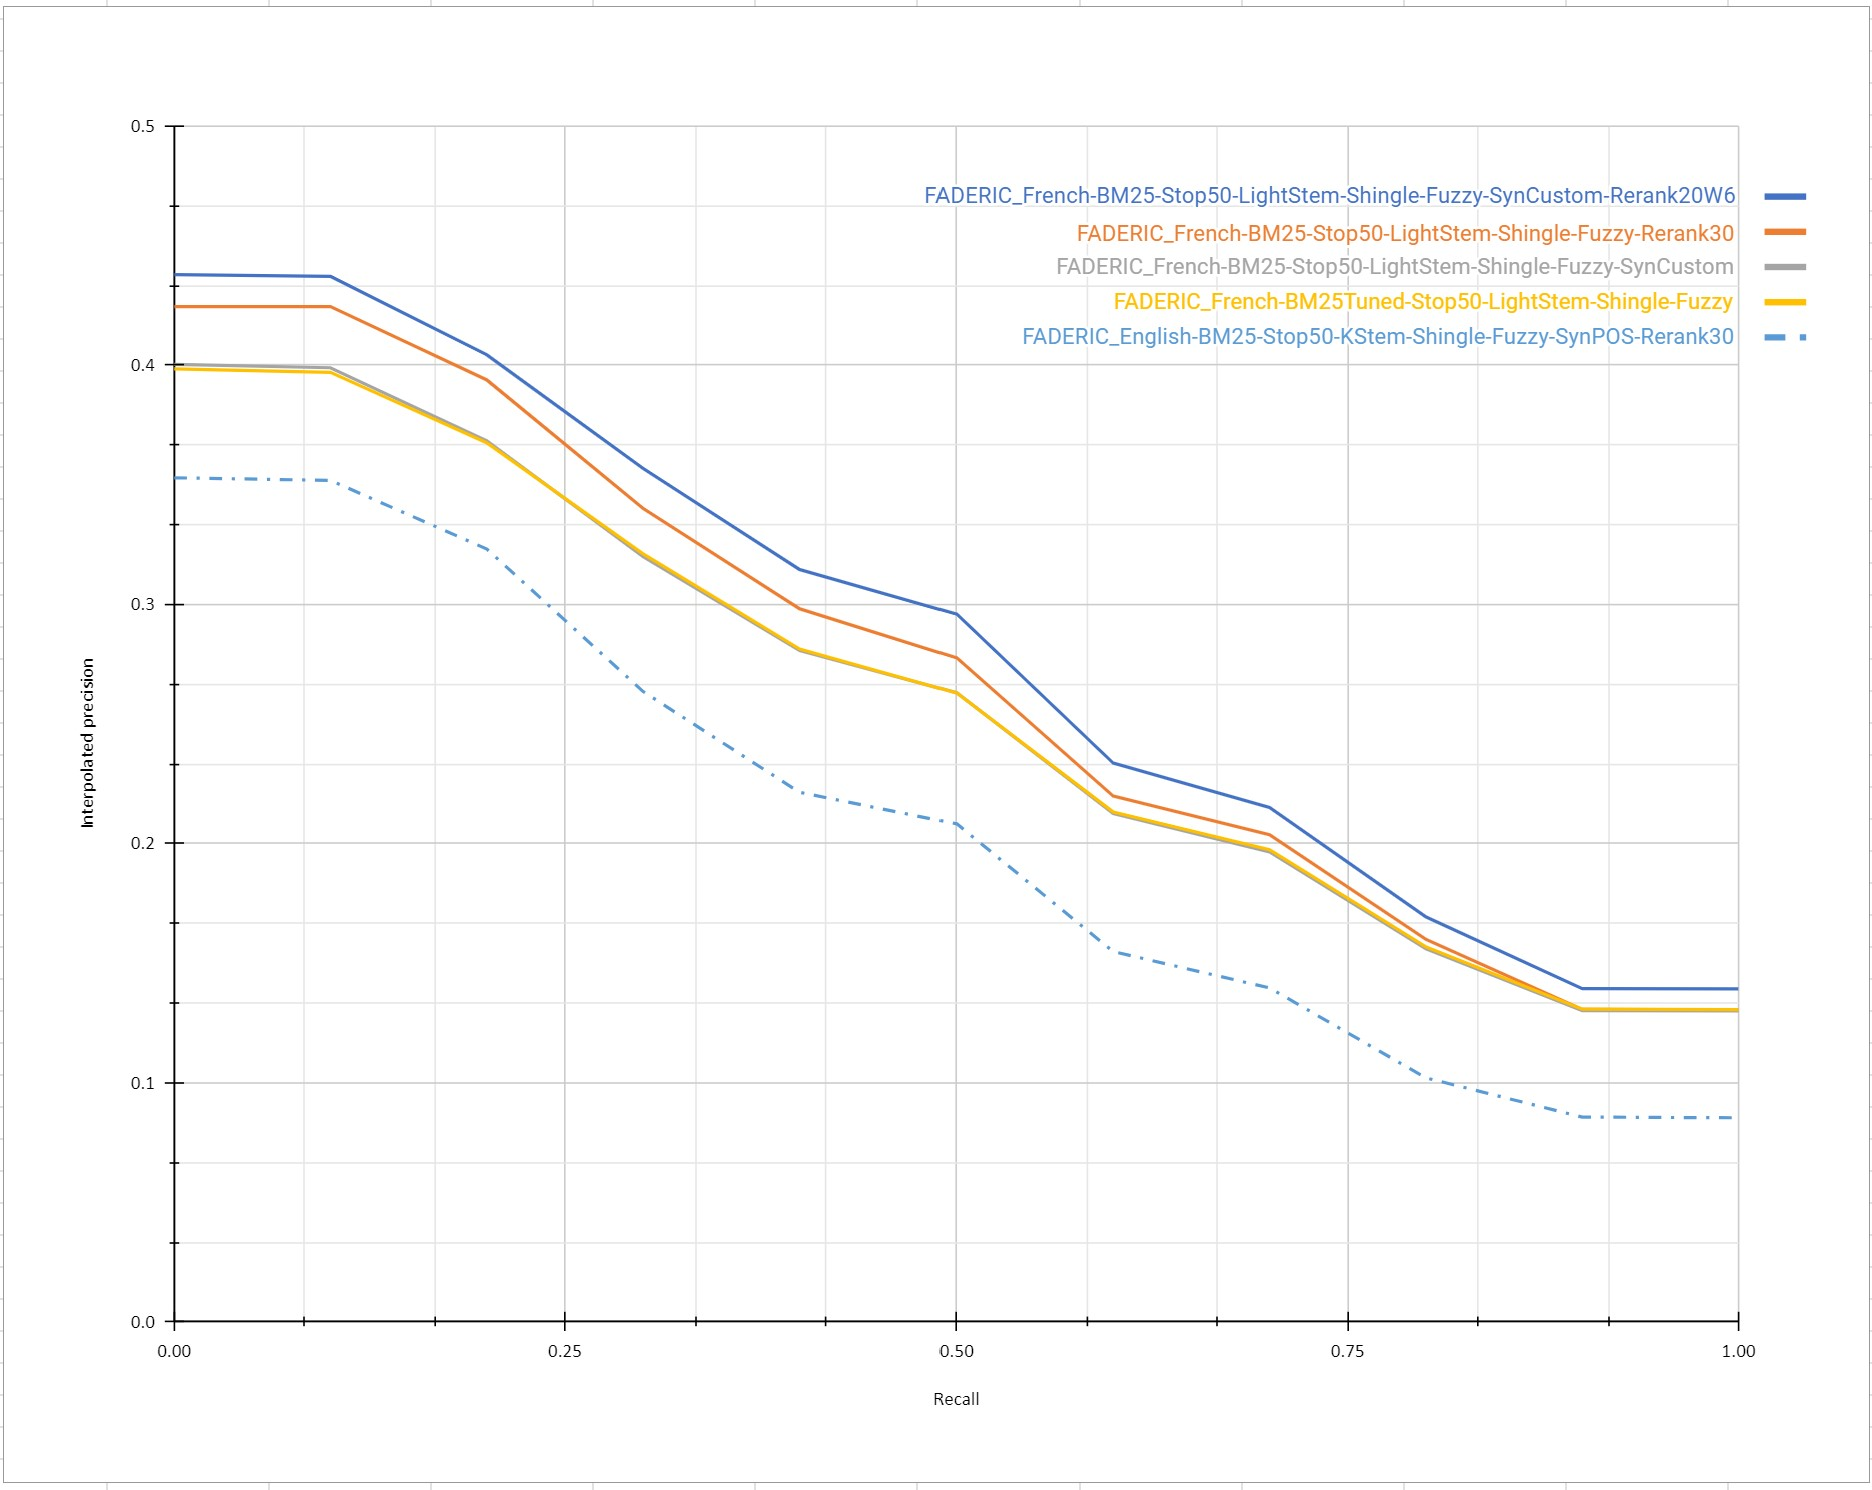
\includegraphics[width=1\linewidth]{figure/iprec-recall-SHORT-TERM.jpg}
  \caption{Interpolated Precision-Recall curve on short term collection}
  \label{fig:precision-recall-curve-short-term}
\end{figure}

\begin{figure}[tbp]
     \centering
     \begin{subfigure}[b]{0.45\textwidth}
         \centering
         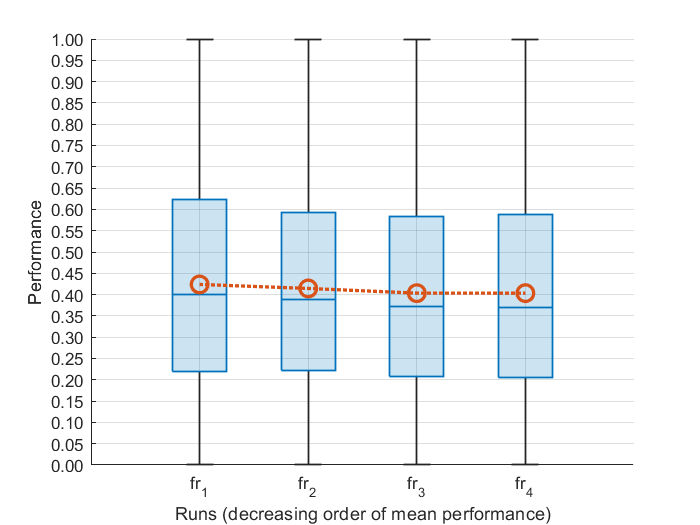
\includegraphics[width=\textwidth]{figure/short-ndcg-boxplot.png}
         \caption{\ac{nDCG}}
     \end{subfigure}
     \hfill
     \begin{subfigure}[b]{0.45\textwidth}
         \centering
         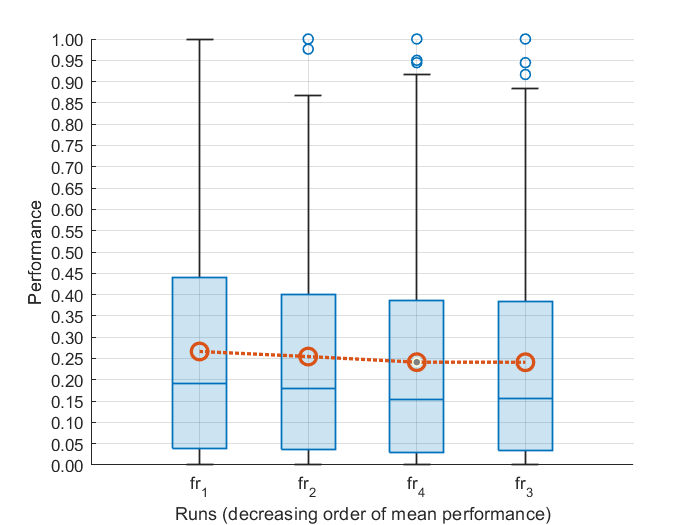
\includegraphics[width=\textwidth]{figure/short-map-boxplot.png}
         \caption{\ac{AP}}
     \end{subfigure}
        \caption{Box plot on short term collection, the mean values are shown in red}
        \label{fig:short-boxplot}
\end{figure}

\begin{table}[tbp]
     \caption{ANOVA2 on short term collection}
    \begin{subtable}[h]{1\textwidth}
        \centering
	 \caption{\ac{nDCG}}
        \begin{tabular}{|l|l|l|l|l|l|}
	\toprule
        \textbf{Source} & \textbf{SS} & \textbf{df} & \textbf{MS} & \textbf{F} & \textbf{Prob$>$F} \\
        \midrule
	\textbf{Systems} & 0.25 & 3  & 0.085  & 13.58  & 8.51E-9 \\
	\textbf{Topics}    & 218.58  & 881  & 0.248 & 39.30 & 0 \\
	\textbf{Error}   & 16.68 & 2643 & 0.006 & - & - \\
	\textbf{Total}   & 235.52  & 3527 & - & - & - \\
	\bottomrule
       \end{tabular}
    \end{subtable}
        \begin{subtable}[h]{1\textwidth}
        \centering
	\caption{\ac{AP}}
        \begin{tabular}{|l|l|l|l|l|l|}
	\toprule
        \textbf{Source} & \textbf{SS} & \textbf{df} & \textbf{MS} & \textbf{F} & \textbf{Prob$>$F} \\
        \midrule
	\textbf{Systems} & 0.38 & 3   & 0.129  & 16.05  & 2.43E-10 \\
	\textbf{Topics}    & 205.64  & 881  & 0.233 & 28.92 & 0 \\
	\textbf{Error}   & 21.32  & 2643 & 0.008 & - & - \\
	\textbf{Total}   & 227.36  & 3527 & - & - & - \\
	\bottomrule
       \end{tabular}
    \end{subtable}
     \label{tab:short-anova2}
\end{table}

\begin{figure}[tbp]
     \centering
     \begin{subfigure}[b]{0.45\textwidth}
         \centering
         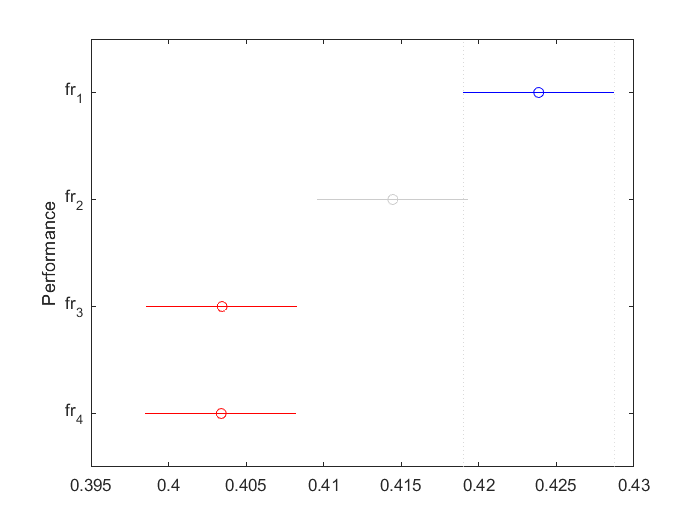
\includegraphics[width=\textwidth]{figure/short-ndcg-hsd.png}
	\caption{\ac{nDCG}}
     \end{subfigure}
     \hfill
     \begin{subfigure}[b]{0.45\textwidth}
         \centering
         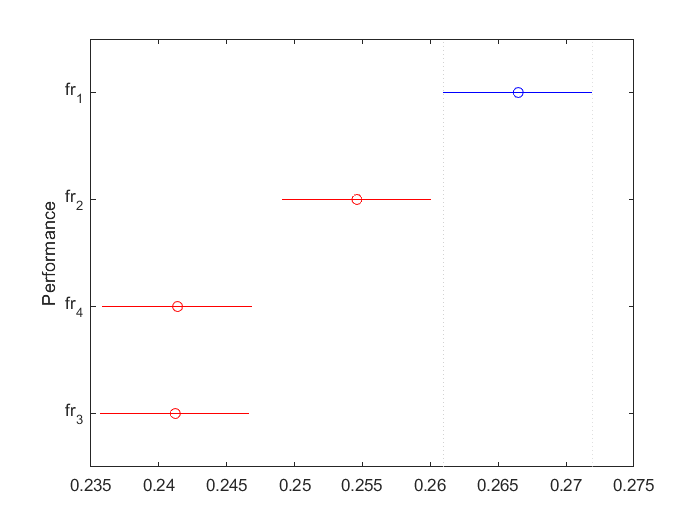
\includegraphics[width=\textwidth]{figure/short-map-hsd.png}
	\caption{\ac{AP}}
     \end{subfigure}
        \caption{Tukey's \ac{HSD} on short term collection}
        \label{fig:short-hsd}
\end{figure}